\documentclass[conference]{IEEEtran}
\IEEEoverridecommandlockouts

\usepackage{cite}
\usepackage{amsmath,amssymb}
\usepackage{graphicx}
\usepackage{booktabs}
\usepackage{multirow}
\usepackage{url}
\usepackage[hidelinks]{hyperref}

\newcommand{\repo}{\url{https://github.com/tali7965/Physics-Constrained-Transformer-for-Motion-Forecasting}}

\begin{document}

\title{Drivable by Construction, Behind on Accuracy:\\
A Kinematic Decoder for Transformer Motion Forecasting on Argoverse~2}

\author{\IEEEauthorblockN{Ali Taheri}
\IEEEauthorblockA{Code and configurations: \repo}}

\maketitle

\begin{abstract}
Most learned motion forecasters regress future coordinates directly, which allows trajectories that
no vehicle could drive. We test the alternative of making every prediction drivable by construction.
The goal is not the most accurate forecaster, but to build a physically accurate one and measure how
it performs. A compact Transformer (1.43M parameters) outputs bounded acceleration and steering, which a
differentiable kinematic bicycle model integrates into positions. We compare it with the same model
using an unconstrained coordinate decoder, under one protocol on Argoverse~2. The kinematic decoder
removes every infeasible trajectory but is less accurate: validation brier-minFDE at $K{=}6$ is
3.16\,m against 2.57\,m. The gap, 0.41--0.73\,m, holds across two seeds, across 10\%, 25\% and
100\% of a 50k-scene training subset, with and without the map, and at $K{=}1$, 3 and 6, so the
physical prior brings no gain in data efficiency. The coordinate decoder's infeasibility is
step-to-step jitter: 58\% of its most probable trajectories exceed 8\,m/s$^2$ of lateral
acceleration at 10\,Hz, and none do at 2\,Hz. The kinematic decoder also leaves the drivable area
more often (5.2\% against 1.5\%). We trace the accuracy gap to the integration, which gives the
first second's controls about 60 times the gradient of the last second's. The off-road excess comes
from errors across the lane: an initial heading the model does not correct, and turns it does not
complete.
\end{abstract}

\section{Introduction}

Motion forecasting predicts where the agents around an autonomous vehicle will be over the next few
seconds. Most current forecasters encode the scene with attention over agents and map
elements~\cite{gao2020vectornet,ngiam2022scenetransformer,nayakanti2023wayformer,shi2022mtr,zhou2023qcnet}
and regress future positions directly. Nothing in such a decoder ties consecutive positions to
vehicle motion, so it can predict sideways slides, turns too sharp for the vehicle's speed, or
jitter between steps. A long-standing remedy is to predict control inputs instead and integrate
them through a vehicle model~\cite{cui2020dkm,salzmann2020trajectronpp}, so that every output is
kinematically feasible by construction. Bounded controls also matter for ride quality: a comfortable
ride avoids heavy steering and harsh acceleration, so it is useful to see how a model limited to
such controls performs.

The goal of this project is not to build the most accurate forecaster, nor to show that a kinematic
decoder is the best approach. It is to build a physically accurate model and measure, in a
controlled setting, what that constraint costs and buys. One Transformer
encoder is trained twice on Argoverse~2~\cite{wilson2021argoverse2}, and only the output head
differs. One head regresses 60 future positions. The other outputs 60 bounded
(acceleration, steering) pairs that a differentiable kinematic bicycle
model~\cite{kong2015kinematic,polack2017kinematic} integrates. Three questions guide the study:
(1)~does the kinematic decoder match the coordinate decoder's accuracy, (2)~how often are
unconstrained trajectories infeasible, and does the kinematic decoder remove them, and (3)~does the
physical prior help more when training data is limited?

The answers are mostly negative for the constrained head, and the reasons are specific:
\begin{itemize}
\item In every setting tested (two seeds, three training-set sizes, with and without the map, and
  three numbers of modes) the kinematic decoder is behind by 0.41--0.73\,m brier-minFDE. That is
  about 40 times the seed-to-seed spread, and the gap does not shrink with less data.
\item The coordinate decoder's infeasibility is almost entirely 10\,Hz jitter. Resampled to 2\,Hz,
  its trajectories are as feasible as the ground truth's or more so.
\item Integration skews the gradient towards early controls by a factor of about 60, and the
  kinematic decoder's accelerations chatter at their bounds. Its off-road excess comes from an
  uncorrected initial heading and from incomplete turns, not from the chatter.
\end{itemize}

\section{Related Work}

\textbf{Scene encoders.} VectorNet~\cite{gao2020vectornet} and LaneGCN~\cite{liang2020lanegcn}
replaced rasterised scenes with vectorised agents and lanes. Transformer forecasters then attend
jointly over agents, time and map~\cite{ngiam2022scenetransformer,nayakanti2023wayformer,shi2022mtr,zhou2023qcnet}.
Ours is a small instance with PointNet-style~\cite{qi2017pointnet} tokens, close to Wayformer's
early-fusion variant~\cite{nayakanti2023wayformer}.

\textbf{Multimodal outputs.} Forecasters predict several modes with probabilities and train them
with a winner-takes-all loss~\cite{guzmanrivera2012mcl}, sometimes around fixed
anchors~\cite{chai2019multipath}. CoverNet~\cite{phanminh2020covernet} classifies over a set of
trajectories that can be made feasible in advance.

\textbf{Kinematic constraints.} DKM~\cite{cui2020dkm} adds a kinematic layer that turns a network's
acceleration and steering outputs into vehicle trajectories. Trajectron++~\cite{salzmann2020trajectronpp}
integrates predicted controls through agent-specific dynamics. The kinematic bicycle model is
standard for planning~\cite{kong2015kinematic} and stays consistent with vehicle motion while
lateral acceleration is moderate~\cite{polack2017kinematic}. We use it in the same way but isolate
its effect: the encoder, losses, data and selection rule are shared, only the head changes, and
feasibility and off-road rates are measured next to accuracy.

\section{Method}

\subsection{Task and data}
Argoverse~2 motion forecasting~\cite{wilson2021argoverse2} gives 5\,s of history for all agents and
a vector map, and asks for the focal agent's next 6\,s at 10\,Hz (60 steps). Each scene is moved to
a frame centred on the focal agent at the last observed step, with the $x$-axis along its recorded
heading. It keeps up to 64 agents and 192 lane segments within 150\,m, each lane as a 10-point
centreline.

\textbf{Protocol.} A seeded permutation of the training split gives a 5,000-scene \emph{dev} set,
used only for model selection, and a fixed 50,000-scene training subset. Its first 10\% and 25\%
form nested subsets for the data-efficiency study. The official validation split (24,988 scenes)
is used only for reporting. The challenge's single-agent leaderboard stopped accepting submissions
on 31 October 2025, so no test results are given.

\subsection{Encoder}
An agent's history steps (position, velocity, $\cos$ and $\sin$ of heading) are embedded linearly,
a learned timestep embedding is added, a LayerNorm--ReLU--Linear block follows, and the result is
max-pooled over valid steps into one token, plus a type embedding. A lane's 9 centreline segments
(start and end points) pass through an MLP and are max-pooled, with lane-type and intersection
embeddings added. A 4-layer pre-norm Transformer encoder~\cite{vaswani2017attention} ($d{=}128$,
8 heads, FFN 512) runs self-attention over all 256 agent and lane tokens, with empty slots masked.
There is no slot positional encoding, so the output does not depend on slot order. $K$ mode
queries, each the focal token plus a learned mode embedding, attend to the scene in a 2-layer
Transformer decoder. An MLP head maps each mode to a trajectory, and a linear layer gives its
logit. The model has 1.43M parameters.

\subsection{Coordinate and kinematic heads}
The \emph{coordinate head} is an MLP that outputs 60 positions per mode.

The \emph{kinematic head} (the physics head in the code) has the same MLP but outputs 60 raw pairs $(u^a_k, u^s_k)$, bounded to an
acceleration $a_k = a_{\max}\tanh u^a_k$ and a steering fraction $s_k = \tanh u^s_k$. Curvature is
$\kappa_k = s_k \min(\kappa_{\max}, a_{\mathrm{lat}}/\bar v_k^2)$: a 5\,m turning radius at low speed
and at most $a_{\mathrm{lat}}$ of lateral acceleration above it. Each step of $\Delta t = 0.1$\,s
integrates
\begin{align}
v_{k+1} &= \max(v_k + a_k \Delta t,\ 0), \quad \bar v_k = \tfrac12 (v_k + v_{k+1}), \nonumber\\
\Delta s_k &= \bar v_k \Delta t, \quad \bar\psi_k = \psi_k + \tfrac12 \kappa_k \Delta s_k, \nonumber\\
(x, y)_{k+1} &= (x, y)_k + \Delta s_k \left(\cos \bar\psi_k, \sin \bar\psi_k\right), \nonumber\\
\psi_{k+1} &= \psi_k + \kappa_k \Delta s_k,
\end{align}
with $a_{\max} = 8$\,m/s$^2$, $\kappa_{\max} = 0.2$\,m$^{-1}$ and $a_{\mathrm{lat}} = 6$\,m/s$^2$.
The initial position is the last observed one. Speed and heading come from the last observed
displacement, or the recorded heading is used below 0.5\,m/s. Every mode is therefore drivable, and
speed cannot become negative. The same head serves every focal type. The bounds cost little
expressiveness: fitting controls directly to 2,000 vehicle-like training futures leaves a mean
endpoint error of 0.16\,m, with 0.55\% of futures more than 2\,m away.

\subsection{Training}
Both heads use a winner-takes-all loss~\cite{guzmanrivera2012mcl}. The mode with the lowest endpoint
error gets the average displacement loss, and the logits get a cross-entropy loss towards that mode;
the two losses are summed. Training uses Adam~\cite{kingma2015adam} with cosine decay, gradient
clipping at 1.0 and batch size 64, for 30 epochs ($\approx$23.5k steps). The learning rates come from
a three-point sweep on the 10\% subset: $10^{-3}$ for the coordinate head, $3\cdot10^{-4}$ for the
kinematic head. The checkpoint with the lowest dev brier-minFDE ($K{=}6$) is kept. A run takes
3.1--3.3\,h on an Apple M4 laptop GPU, with the training subset held in memory. The data-efficiency
runs keep the number of gradient steps fixed at $\approx$23.5k (300, 120 and 30 epochs) and check dev
every $\approx$790 steps.

\subsection{Metrics}
Accuracy follows the Argoverse~2 definitions. Among the $K$ most probable modes, the one with the
lowest endpoint error is scored: minADE and minFDE are its mean and final errors, a miss (MR) is a
minFDE above 2\,m, and brier-minFDE adds $(1-p)^2$ for that mode's probability $p$. At $K{=}1$ the
most probable mode is scored. Our implementation matches the \texttt{av2} package's functions.
Physical plausibility is measured for vehicle-like focal agents (vehicle, bus, motorcyclist). A
trajectory is \emph{infeasible} if its lateral acceleration (speed times yaw rate) exceeds
8\,m/s$^2$ at any step while moving faster than 1\,m/s. This is checked at 10\,Hz and on the
trajectory resampled to 2\,Hz, which judges the manoeuvre rather than step-to-step noise. A
trajectory is \emph{off-road} if any point lies outside every drivable-area polygon of the
scenario's map. ``@1'' is the most probable mode and ``@6'' covers all modes.

\section{Results}

\begin{table}[t]
\centering
\caption{Validation results, all 24,988 focal agents. $K{=}1$ scores the most probable mode;
``brier'' is brier-minFDE, the leaderboard metric.}
\label{tab:main}
\footnotesize
\setlength{\tabcolsep}{2.3pt}
\begin{tabular}{lccccccc}
\toprule
& \multicolumn{3}{c}{$K{=}1$} & \multicolumn{4}{c}{$K{=}6$} \\
\cmidrule(lr){2-4}\cmidrule(lr){5-8}
Model & minADE & minFDE & MR & minADE & minFDE & MR & brier \\
\midrule
Constant velocity & 4.40 & 11.66 & .855 & -- & -- & -- & -- \\
LSTM~\cite{hochreiter1997lstm} & 3.15 & 8.33 & .821 & -- & -- & -- & -- \\
Coordinate head & \textbf{2.45} & \textbf{6.09} & \textbf{.709} & \textbf{1.06} & \textbf{1.94} & \textbf{.303} & \textbf{2.57} \\
Kinematic head & 2.74 & 6.95 & .755 & 1.25 & 2.55 & .431 & 3.16 \\
\bottomrule
\end{tabular}
\end{table}

\begin{table}[t]
\centering
\caption{Physical plausibility on validation, vehicle-like focal agents (23,113): share of
trajectories, most probable mode / all six modes.}
\label{tab:plaus}
\setlength{\tabcolsep}{4pt}
\begin{tabular}{lccc}
\toprule
& Infeasible, 10\,Hz & Infeasible, 2\,Hz & Off-road \\
\midrule
Ground truth & 2.93\% & 0.41\% & 0.19\% \\
Coordinate head & 57.8 / 70.0\% & 0.00 / 0.01\% & \textbf{1.52 / 1.75\%} \\
Kinematic head & \textbf{0.00 / 0.00\%} & \textbf{0.00 / 0.00\%} & 5.17 / 5.68\% \\
\bottomrule
\end{tabular}
\end{table}

\subsection{Accuracy and feasibility}
Table~\ref{tab:main} gives the main comparison. The Transformer with the coordinate head is 22\%
better than a focal-history LSTM~\cite{hochreiter1997lstm} on $K{=}1$ minADE and 27\% better on
minFDE. The kinematic head is behind the coordinate head on every metric: brier-minFDE is 3.16
against 2.57, and $K{=}1$ minFDE is 6.95 against 6.09. It still beats the LSTM. Pedestrians do not
explain the gap: for vehicle-like agents brier-minFDE is 3.28 against 2.64.

Table~\ref{tab:plaus} answers the feasibility question. At 10\,Hz, 58\% of the coordinate head's
most probable trajectories break the lateral-acceleration limit. At that rate a $\pm$4\,cm zigzag
between steps already exceeds 8\,m/s$^2$, and even the tracked ground truth fails 2.9\% of the
time. Resampled to 2\,Hz, the coordinate head is at 0.00\%, against 0.41\% for the ground truth:
its manoeuvres are feasible, and its 10\,Hz infeasibility is jitter. The kinematic head is 0.00\%
infeasible at both rates, as built. But it leaves the drivable area more than three times as often
(5.2\% against 1.5\%).

\subsection{Ablations}

\begin{table}[t]
\centering
\caption{Ablations on validation. brier-minFDE at the model's own $K$ (all focal agents; for
$K{=}1$, minFDE) and off-road for the most probable mode (vehicle-like). Gaps are computed from
unrounded values.}
\label{tab:ablate}
\setlength{\tabcolsep}{3.5pt}
\begin{tabular}{lccccc}
\toprule
& \multicolumn{3}{c}{brier-minFDE (m)} & \multicolumn{2}{c}{Off-road @1} \\
\cmidrule(lr){2-4}\cmidrule(lr){5-6}
Setting & Coord. & Kinem. & Gap & Coord. & Kinem. \\
\midrule
100\%, $K{=}6$, seed 0 & 2.57 & 3.16 & 0.59 & 1.5\% & 5.2\% \\
100\%, $K{=}6$, seed 1 & 2.56 & 3.18 & 0.62 & 1.6\% & 5.9\% \\
25\% (12.5k scenes) & 2.88 & 3.61 & 0.73 & 2.3\% & 7.9\% \\
10\% (5k scenes) & 3.33 & 3.98 & 0.66 & 4.1\% & 8.1\% \\
No map & 3.18 & 3.58 & 0.41 & 4.0\% & 7.1\% \\
$K{=}3$ & 3.17 & 3.72 & 0.54 & 1.6\% & 4.7\% \\
$K{=}1$ & 5.19 & 5.81 & 0.62 & 2.0\% & 4.6\% \\
\bottomrule
\end{tabular}
\end{table}

\begin{figure}[t]
\centering
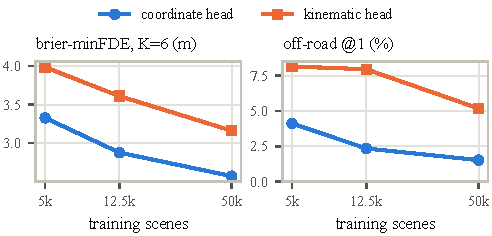
\includegraphics[width=\columnwidth]{figures/data_efficiency.pdf}
\caption{Data efficiency on validation. Every run gets $\approx$23.5k gradient steps, so smaller
subsets get more epochs. The kinematic head's gap does not shrink with less data.}
\label{fig:data}
\end{figure}

Table~\ref{tab:ablate} varies one setting at a time, each a separate pair of training runs.

\textbf{Seeds.} A second seed moves each head's brier-minFDE by at most 0.016\,m, while the gap is
0.59 and 0.62\,m.

\textbf{Data efficiency.} The gap is 0.66\,m at 10\%, 0.73\,m at 25\% and 0.59\,m at 100\%, or 20--25\%
of the coordinate head's error (Fig.~\ref{fig:data}). The kinematic head trained on 50k scenes is
behind the coordinate head trained on 12.5k. The one exception is the most probable mode at 10\%,
where the kinematic head is slightly ahead ($K{=}1$ minFDE 8.51 against 8.62). Both heads overfit
the small subsets, the kinematic head earlier and further: at 10\% its dev brier-minFDE rises from
4.02 at epoch 80 to 5.25 at epoch 300. Its training displacement error then falls to 0.73\,m, the
same as the coordinate head's 0.74\,m and far below the 1.18\,m at which the full kinematic run
ends. Given enough passes, it fits its training scenes as well as the coordinate head does, so the
full-data gap reflects slow optimisation rather than missing expressiveness. The coordinate head's
jitter, meanwhile, grows as data shrinks: 97\% of its most probable trajectories are infeasible at
10\,Hz when trained on 10\%.

\textbf{Map.} Removing the lane tokens costs the coordinate head 0.60\,m and the kinematic head
0.42\,m. The gap shrinks to 0.41\,m but remains, so a weaker use of the map explains only part of
it. With the map, the kinematic head still leaves the road more often than the coordinate head
does without one (5.2\% against 4.0\%).

\textbf{Number of modes.} Models trained with $K{=}1$ and $K{=}3$ are selected on dev minFDE and
brier-minFDE at $K{=}3$, respectively. The gap is 0.62, 0.54 and 0.59\,m at $K{=}1$, 3 and 6. A single-mode model
predicts better than a six-mode model's most probable mode (5.19 against 6.09 for the coordinate
head, 5.81 against 6.95 for the kinematic head), so mode scoring is a weak point of both $K{=}6$
models.

\section{Diagnosis}

The following analyses compare the two full-data checkpoints on the dev set.

\subsection{Why the kinematic head is less accurate}

\begin{figure}[t]
\centering
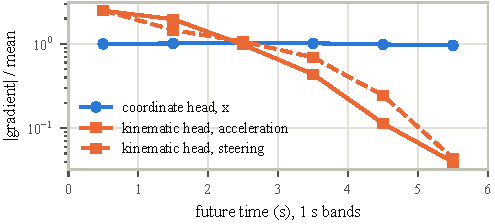
\includegraphics[width=\columnwidth]{figures/gradient.pdf}
\caption{Mean $|\partial \mathcal{L} / \partial \text{head output}|$ per 1\,s band of the future,
relative to its mean over all 60 steps (dev, training loss). A control moves every later position,
so integration makes the first second's controls receive about 60 times the gradient of the last
second's.}
\label{fig:grad}
\end{figure}

\textbf{Late controls get little gradient.} Fig.~\ref{fig:grad} shows how the training loss's
gradient reaches the head's outputs. For the coordinate head it is flat over the horizon. For the
kinematic head it falls from 2.5 times the mean in the first second to 0.04 times in the last, for
both acceleration and steering. This is an effect of integrating through time, akin to the
gradient problems of recurrent networks~\cite{pascanu2013difficulty}. The best-of-six error gap
grows with the horizon accordingly: 0.16\,m at 3\,s, 0.46\,m at 5\,s and 0.65\,m at 6\,s.

\textbf{Accelerations chatter at their bounds.} In the most probable mode, 31\% of accelerations lie
within 5\% of $\pm 8$\,m/s$^2$ (55\% in the last 2\,s), against 6\% of steering values. In the first
4\,s the acceleration changes sign at 57--80\% of steps. Over 1\,s windows, though, it averages out
close to the ground truth (median $|a|$ 0.88 against 0.61\,m/s$^2$). Where $\tanh$ saturates, little
gradient passes. Forcing smooth controls does not help: knots every 0.5\,s with linear
interpolation remove the chatter by construction and raise the fitting floor only from 0.16 to
0.17\,m. On the 10\% subset (30 epochs), however, dev brier-minFDE is worse with knots at both
seeds (4.41 and 4.21 against 4.28 and 4.13). The imbalance comes from integration, not from the
chatter.

\textbf{The ground truth ends with an artifact.} Over the last 0.7\,s, the focal agent's ground-truth
positions slow down sharply while its recorded velocity does not. Vehicle-like speed from position
differences falls from 7.7 to 3.6\,m/s, an apparent $-8.6$\,m/s$^2$ at the last step. The artifact is
present in the raw data. A coordinate head can copy it, while the kinematic head would have to
brake at its bound. It accounts for only about 0.1\,m of the gap, however: the gap grows at the same
rate before and after it begins.

\subsection{Why the kinematic head leaves the road}

\begin{table}[t]
\centering
\caption{Off-road share of the most probable mode on dev, vehicle-like agents (4,636), by
condition. Heading change: first against last 1\,s chord of the ground truth. $e_0$: angle between
the kinematic head's initial heading and the ground truth's first-second direction. Lateral miss:
endpoint error across the ground truth's final direction (scene counts differ per head).}
\label{tab:offroad}
\setlength{\tabcolsep}{4pt}
\begin{tabular}{lccc}
\toprule
Condition & Scenes & Coord. & Kinem. \\
\midrule
All & 4,636 & 1.6\% & 5.2\% \\
Straight ($<10^\circ$), $|e_0| < 1^\circ$ & 2,016 & 0.2\% & 1.2\% \\
Straight ($<10^\circ$), $|e_0| \ge 4^\circ$ & 125 & 2.4\% & 18.4\% \\
Bend ($10$--$30^\circ$) & 305 & 4.6\% & 14.8\% \\
Turn ($\ge 30^\circ$) & 584 & 6.8\% & 18.2\% \\
Lateral miss 2--4\,m & 362 / 491 & 5.5\% & 10.6\% \\
Lateral miss $\ge 4$\,m & 295 / 516 & 9.2\% & 28.3\% \\
\bottomrule
\end{tabular}
\end{table}

\begin{figure*}[t]
\centering
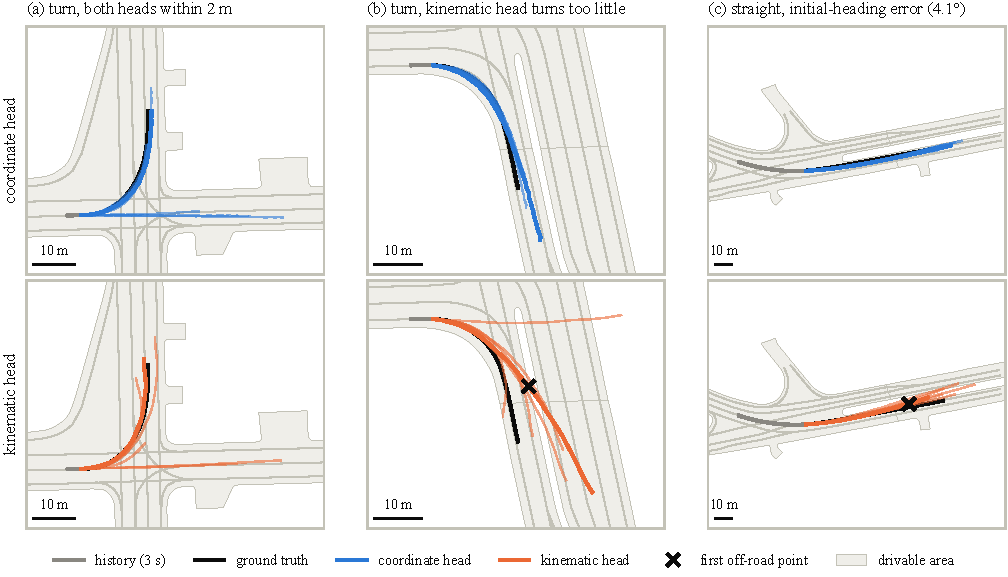
\includegraphics[width=\textwidth]{figures/examples.pdf}
\caption{Dev scenes, each drawn at random from the scenes that meet its condition. Thick lines are
the most probable modes. (a)~A turn in which both heads' most probable modes end within 2\,m (one of
3). (b)~A turn in which the kinematic head's most probable mode turns the right way but only
25--75\% as far, and leaves the road while the coordinate head's stays on it (one of 19).
(c)~A straight road on which the kinematic head starts $4.1^\circ$ off the ground truth's direction
and keeps that heading across the median (one of 21). Panels (b) and (c) show failure modes, not
how often they occur: overall, the kinematic head's most probable mode stays on the road in about
95\% of vehicle-like scenes (5.2\% off-road on both dev and validation).}
\label{fig:examples}
\end{figure*}

Table~\ref{tab:offroad} and Fig.~\ref{fig:examples} locate the off-road excess.

\textbf{Drivable is not road-aware.} The bicycle model limits how the vehicle moves, not where it may
go: a smooth, drivable path can still cross a median. Staying on the road is learned from the map,
by both heads alike. What the constraint changes is how errors build up. The coordinate head places
each point directly and can follow the lane's shape point by point. The kinematic head's position is
the running sum of its controls, so a small early error in heading or steering compounds into a
smooth drift across the lane.

\textbf{Not the chatter.} Re-rolling the kinematic head's own controls after a 1\,s moving average
gives 5.0\% off-road instead of 5.2\%. Removing its steering in the last second gives 5.5\%.

\textbf{Mostly turns.} Futures that change heading by $10^\circ$ or more are 19\% of the scenes but
62\% of the kinematic head's off-road modes. Its most probable mode turns less than the ground
truth (median 0.85 of the heading change, against 0.92 for the coordinate head), and 61\% of its
off-road modes in turns end on the outside of the turn (coordinate head 55\%). The bounds are not
what stops it: its best mode turns as far as the coordinate head's (0.92 against 0.94), and in the
turns where it leaves the road its steering is at the bound in only 18\% of steps. The accuracy gap
has the same shape: on dev, brier-minFDE trails by 0.68\,m on straight roads and by 1.1\,m in bends
and turns.

\textbf{Uncorrected initial heading.} On straight roads, over its first second, the kinematic head's
most probable mode keeps 94\% of the error $e_0$ in its initial heading, where the coordinate head
keeps 3\%. Its starting heading, the last-step displacement, is the better of the two available
(closer to the first ground-truth step than the recorded heading), but the head does not correct
what error remains. Its off-road share on straight roads rises
from 1.2\% for $|e_0| < 1^\circ$ to 18.4\% for $|e_0| \ge 4^\circ$ (coordinate head: 0.2\% to 2.4\%).

\textbf{Errors across the lane.} When the most probable mode misses the ground truth's endpoint by
more than 2\,m sideways, the kinematic head leaves the road 2--3 times as often as the coordinate
head with the same miss.

\section{Discussion and Limitations}

For this encoder and benchmark, hard per-step kinematic decoding has a clear cost and a small
benefit. The cost is 0.4--0.7\,m of brier-minFDE in every setting, with no gain in data efficiency.
The benefit is the removal of 10\,Hz jitter; the coordinate head's manoeuvres are already feasible
at 2\,Hz. The kinematic head can fit futures within 0.16\,m and, given enough passes, fits its
training scenes as well as the coordinate head. Its problems are therefore optimisation and initial
state, not capacity. These point to remedies we have not tested: rescaling the gradient per step,
predicting controls as residuals around a lane-following reference, estimating the initial state
from more of the history, or projecting a coordinate decoder's output onto feasible trajectories
instead of decoding controls directly. The bounds here reach nearly every real future, so they rule
out extreme manoeuvres rather than enforce comfort; a comfort-oriented model would tighten them and
limit how fast steering may change.

\textbf{A hybrid decoder.} The kinematic head's failures concentrate in sharp turns: it leaves the
road in 2.4\% of straight-road scenes (coordinate head 0.5\%) but in 18.2\% of turns of $30^\circ$ or
more (6.8\%). This suggests a hybrid that decodes kinematically on straight roads and gentle
curves, where smooth, drivable output is cheap, and with coordinates in sharp turns. Two
conditions would decide whether it pays off. The switch must use information available at
prediction time, such as the lane geometry ahead, rather than the ground-truth turn used here.
And the kinematic head's 0.68\,m gap on straight roads, mostly its uncorrected initial heading,
would need closing too. We leave this open for future work.

The study has clear limits. It uses one small model (1.43M parameters), a 50k-scene training
subset, one benchmark and two seeds for the main comparison. Results are on validation only, because
the leaderboard had closed. Learning rates come from a three-point sweep on the 10\% subset. The
kinematic head also serves pedestrians, although the gap is the same for vehicle-like agents. The
diagnoses use one checkpoint per head. Off-road depends on the map's drivable-area polygons.

\section{Conclusion}

This project set out to build a physically accurate forecaster and measure how it performs, not to
find the best approach. Integrating bounded controls through a kinematic bicycle model makes every
trajectory drivable, but on Argoverse~2 it costs 0.4--0.7\,m in every setting and does not improve
data efficiency. Correcting the initial heading and the slow learning of late controls, rather than
adding constraints, is the natural next step.

\bibliographystyle{IEEEtran}
\bibliography{references}

\end{document}
